\chapter{TINJAUAN PUSTAKA}
\label{chap:tinjauanpustaka}

% Ubah bagian-bagian berikut dengan isi dari tinjauan pustaka
% Demi mendukung penelitian ini, \lipsum[1][1-5]

\section{Hasil Penelitian Terdahulu}
\label{sec:hasilpenelitianterdahulu}
Adapun penulis mengambil beberapa penelitian terdahulu yang mengambil topik yang sama ataupun beririsan sebagai referensi, serta dasar pengembangan dan inovasi yang akan pada tugas akhir ini. Berikut adalah beberapa penelitian terdahulu yang diambil sebagai referensi:

\subsection{Deteksi Kendaraan Truk pada Video Menggunakan Metode Tiny-YOLOv4}
\label{subsec:deteksikendaraantrukprismadika}
Penelitian oleh Prismadika Yuniar et al. \parencite*{prismadika2023} mengkaji deteksi truk secara real-time dalam video pengamatan di jalan raya. Tantangan muncul karena truk memiliki dimensi serupa dengan bus dan struktur mekanis mirip pikap. Pada tahap awal, model YOLO asli hanya mampu mendeteksi bagian kepala dan bak truk tanpa memperhitungkan muatan. Oleh karena itu, dibuat custom dataset dengan bounding box untuk seluruh bagian truk beserta muatannya.

Tiny-YOLOv4 dipilih karena lebih ringan dan kompatibel dengan perangkat beragam. Pengujian pada tiga perangkat menunjukkan bahwa Laptop Acer E5 mencapai akurasi 98,2\% pada 13 FPS, Laptop Lenovo Legion 5 98\% pada 28 FPS, dan PC Dell Precision 3640 Tower 97,5\% pada 38 FPS. 

Hasil yang didapatkan yaitu FPS yang lebih tinggi cenderung menurunkan akurasi, dan perangkat dengan CPU di atas 3.0 GHz, RAM minimal 16 GB, dan GPU lebih dari 4 GB mampu menjalankan deteksi secara real-time dengan baik.

\subsection{Sistem Deteksi Kendaraan Overdimension secara Real-time menggunakan Deep Learning di Jalan Raya}
\label{subsec:deteksikendaraanoverdimensionhamayan}
Penelitian ini dilakukan oleh Ahmad Hamayan Nabih \parencite*{hamayan2024}. Penelitian ini bertujuan untuk mengembangkan sistem deteksi kendaraan overdimension secara real-time menggunakan deep learning di jalan raya. Sistem ini menggunakan model YOLOv8 yang telah dimodifikasi untuk mendeteksi kendaraan overdimension. Dataset yang digunakan adalah dataset yang telah diambil dari jalan raya di Indonesia. Variasi yang digunakan yaitu variasi akurasi pada berbagai macam perangkat dan model YOLOv8.

Variasi perangkat meliputi PC dengan External VGA NVIDIA GeForce GTX 1650Ti, Laptop tanpa External VGA, dan Intel NUC i5 Gen 11. Hasil yang didapatkan yaitu PC dengan External VGA NVIDIA GeForce GTX 1650Ti mampu mendeteksi kendaraan overdimension dengan akurasi 85\% - 90\% pada 33 FPS - 63 FPS, Laptop tanpa External VGA dengan akurasi 87\% - 92\% pada 7 FPS - 10 FPS, dan Intel NUC i5 Gen 11 dengan akurasi 79\% - 90\% pada 2 FPS. Sedangkan variasi model YOLOv8 meliputi YOLOv8n dan YOLOv8s, dimana YOLOv8n di-\emph{training} dengan 50 \emph{epoch} dan YOLOv8s di-\emph{training} dengan 75 \emph{epoch}.

Kesimpulan yang didapatkan yaitu model YOLOv8n lebih baik dari segi FPS dibandingkan dengan YOLOv8s namun memiliki akurasi yang lebih rendah. Sedangkan model pembandingnya, yaitu YOLOv8s memiliki akurasi yang lebih tinggi namun FPS yang lebih rendah. Kemudian juga ditemukan bahwa perangkat dengan spesifikasi yang lebih tinggi mampu mendeteksi kendaraan overdimension dengan akurasi yang lebih tinggi dan FPS yang lebih tinggi.

\subsection{Implementasi Sistem Penghitung Kendaraan Otomatis Berbasis Computer Vision}
\label{subsec:implementasisistemhitungkendaraan}
Penelitian ini dilakukan oleh Dolly Indra et al. \parencite*{dolly2023}. Penelitian ini bertujuan untuk mengembangkan sistem penghitung kendaraan otomatis di tempat pencucian kendaraan. Sistem ini menggunakan Raspberry Pi 4 sebagai \emph{edge device} dan model SSD MobileNet V2 sebagai model deteksi. Sistem ini mampu menghitung jumlah kendaraan yang masuk dan keluar dari tempat pencucian kendaraan secara realtime yang terhubung dengan aplikasi \emph{mobile}.

Hasil yang didapatkan yaitu sistem otomatis mampu mendeteksi kendaraan mobil dan motor dengan rata-rata tingkat akurasi sebesar 46,6 \% dan aplikasi yang terdapat pada \emph{smartphone} mampu menghitung jumlah kendaraan yang masuk dan keluar dari tempat pencucian kendaraan.

\section{Teori/Konsep Dasar}
\label{sec:teorikonsepdasar}
Adapun berikut adalah teori atau konsep dasar yang digunakan penulis sebagai landasan teoritis dalam pelaksanaan tugas akhir ini.

\subsection{CNN (\emph{Convolutional Neural Network})}
\emph{Convolutional Neural Networks} (CNN) merupakan salah satu arsitektur deep learning yang paling banyak digunakan dalam pengolahan citra. CNN pertama kali diperkenalkan oleh Yan LeCun et al. \parencite*{yannlecun1998} dalam penelitian tentang pengenalan tulisan tangan menggunakan LeNet-5. Model ini menggabungkan operasi konvolusi, \emph{subsampling} (\emph{pooling}), dan \emph{fully connected layers} untuk mengekstraksi fitur secara hierarkis dari gambar input.

Perkembangan CNN semakin pesat dengan adanya inovasi pada arsitektur. Salah satu inovasi signifikan adalah Residual Neural Network (ResNet) yang diperkenalkan oleh Kaiming He et al. \parencite*{kaiminghe2015}. ResNet memperkenalkan konsep \emph{skip connection} yang memungkinkan model untuk belajar representasi yang lebih baik dari data. Hal ini memungkinkan model untuk dilatih dengan kedalaman yang lebih besar tanpa mengalami masalah \emph{vanishing gradient}.

Selain itu, metode modern seperti normalisasi batch (\emph{BatchNorm}) yang dikembangkan oleh Ioffe et al. \parencite*{ioffe2015} dan Szegedy et al. \parencite*{szegedy2015} telah menjadi standar dalam pelatihan CNN. \emph{BatchNorm} membantu jaringan untuk melakukan konvergensi lebih cepat dengan menormalkan distribusi setiap batch selama pelatihan. Penggunaan konvolusi 1x1, seperti pada arsitektur \emph{Inception}, juga memperkenalkan cara baru untuk mengurangi jumlah parameter sambil mempertahankan kapasitas jaringan.

Penerapan CNN telah meluas ke berbagai domain, termasuk deteksi objek, segmentasi citra, dan pengenalan pola. Dalam konteks penelitian ini, CNN digunakan untuk mendeteksi kendaraan overdimensi berdasarkan karakteristik visualnya. Pendekatan ini sesuai dengan studi sebelumnya yang menunjukkan kemampuan CNN dalam mengolah data visual dengan tingkat akurasi yang tinggi.

\subsection{SSD (\emph{Single Shot MultiBox Detector})}

\emph{Single Shot MultiBox Detector} (SSD) adalah arsitektur deteksi objek yang dikembangkan oleh Liu et al. \parencite*{liu2016}. SSD memperkenalkan pendekatan \emph{single shot} yang memungkinkan model untuk melakukan deteksi objek dan klasifikasi dalam satu langkah. Hal ini berbeda dengan pendekatan \emph{two-stage} seperti Faster R-CNN yang memerlukan dua tahap untuk deteksi objek.

SSD menggunakan \emph{multi-scale feature maps} untuk mendeteksi objek pada berbagai skala. Arsitektur ini terdiri dari \emph{base network} (biasanya menggunakan arsitektur VGG16 atau ResNet) yang diikuti oleh beberapa lapisan konvolusi untuk menghasilkan \emph{feature maps} pada berbagai resolusi. Setiap lapisan \emph{feature map} digunakan untuk memprediksi kotak pembatas (\emph{bounding box}) dan kelas objek yang terdapat dalam gambar.

SSD telah terbukti efektif dalam deteksi objek pada berbagai dataset, termasuk PASCAL VOC dan COCO. Keunggulan utama SSD adalah kemampuannya untuk melakukan deteksi objek secara cepat dan akurat dalam satu langkah. Dalam konteks penelitian ini, SSD digunakan sebagai model deteksi untuk mengidentifikasi kendaraan overdimensi pada video pengamatan jalan raya.

\subsection{Edge Computing}

Edge computing adalah paradigma komputasi yang memungkinkan pemrosesan data dilakukan di dekat sumber data, seperti perangkat IoT atau sensor. Hal ini bertentangan dengan komputasi tradisional yang memerlukan pengiriman data ke pusat data atau cloud untuk diproses. Edge computing memungkinkan pemrosesan data yang lebih cepat, responsif, dan efisien dengan memanfaatkan sumber daya lokal.

Keuntungan utama dari edge computing adalah kemampuannya untuk mengurangi latensi dan mempercepat respons sistem \parencite*{aws2024}. Dengan melakukan pemrosesan data di dekat sumber data, edge computing memungkinkan aplikasi untuk merespons lebih cepat terhadap perubahan kondisi lingkungan. Hal ini sangat penting dalam konteks aplikasi real-time seperti deteksi objek pada video pengamatan jalan raya.

Selain itu, edge computing juga membantu mengurangi beban jaringan dan cloud dengan melakukan pemrosesan data secara lokal. Hal ini dapat mengurangi biaya operasional dan meningkatkan efisiensi sistem secara keseluruhan. Dalam konteks penelitian ini, edge computing digunakan untuk menjalankan model deteksi objek secara real-time pada perangkat lokal tanpa memerlukan koneksi internet. 

Contoh implementasi edge computing yang digunakan dalam penelitian ini adalah Jetson Nano dan Beelink Gemini T34  yang berfungsi sebagai edge device untuk menjalankan model deteksi objek secara real-time.


\subsection{Flutter}

Flutter adalah \emph{framework} pengembangan aplikasi \emph{open-source} yang dikembangkan oleh Google \parencite*{google2024}. Flutter memungkinkan pengembang untuk membuat aplikasi mobile dengan antarmuka pengguna yang kaya dan responsif. Flutter menggunakan bahasa pemrograman Dart yang dikembangkan oleh Google sebagai bahasa utamanya.

Keunggulan utama dari Flutter adalah kemampuannya untuk membuat aplikasi mobile yang konsisten di berbagai platform, termasuk Android dan iOS. Flutter menggunakan \emph{widget} sebagai komponen dasar untuk membangun antarmuka pengguna. \emph{Widget} Flutter bersifat deklaratif, yang berarti pengembang mendefinisikan bagaimana antarmuka pengguna harus terlihat berdasarkan kondisi saat ini.

Flutter juga menyediakan berbagai \emph{plugin} dan \emph{package} yang memperluas fungsionalitas aplikasi. Pengembang dapat menggunakan \emph{plugin} Flutter untuk mengakses fitur perangkat seperti kamera, lokasi, dan sensor. Selain itu, Flutter juga menyediakan \emph{package} untuk mengintegrasikan aplikasi dengan layanan cloud, database, dan API eksternal.

Dalam konteks penelitian ini, Flutter digunakan sebagai platform pengembangan aplikasi mobile untuk menampilkan hasil deteksi objek secara real-time. Aplikasi Flutter akan berkomunikasi dengan edge device untuk menerima data deteksi objek dan menampilkannya dalam antarmuka pengguna yang responsif.

% \subsection{Tunarungu} 
% % \label{sec:gravitasi}

% Tunarungu merupakan suatu istilah yang digunakan untuk menjelaskan kondisi seseorang yang kehilangan atau ketidakmampuan seseorang dalam menangkap rangsangan secara auditori melalui indra pendengarannya \parencite{somantri2006}. Apabila ditinjau dari segi kelahiran, tunarungu dapat dibagi menjadi dua, yaitu \emph{congentially deaf} (ketidakmampuan dengar yang terjadi sejak awal kelahiran) dan \emph{adventitiously deaf} (ketidakmampuan dengar yang terjadi karena penyakit atau peristiwa traumatis yang terjadi pada individu dengan kelahiran tanpa adanya riwayat gangguan pendengaran) \parencite{hallahan2009}. Tunarungu juga dapat dibedakan berdasarkan tingkat kemampuan pendengaran yang dinyatakan dalam intensitas suara yang didengar dengan satuan dB (decibel), yaitu kelompok I (kehilangan 15-30 dB) atau \emph{mild hearing losses} (ketunarunguan ringan), kelompok II kehilangan (31-60 dB) atau \emph{moderate hearing losses} (ketunarunguan sedang), kelompok II (kehilangan 61-90 dB) atau \emph{severe hearing losses} (ketunarunguan berat), kelompok IV (kehilangan 91-120 dB) atau \emph{profound hearing losses} (ketunarunguan sangat berat), dan kelompok V (kehilangan lebih dari 120 dB) atau \emph{total hearing losses} (ketunarunguan total) \parencite{winarsih2007}. Di Indonesia, tercatat terdapat setidaknya 2,9 juta atau setidaknya 1,25\% penduduk Indonesia yang merupakan penyandang tunarungu \parencite{evitasari2015}. Angka ini terbilang cukup besar jika dibandingkan dengan keseluruhan penduduk Indonesia.

% \subsection{Bahasa Isyarat Indonesia (BISINDO)}
% \begin{figure}[H]
%     \centering

%     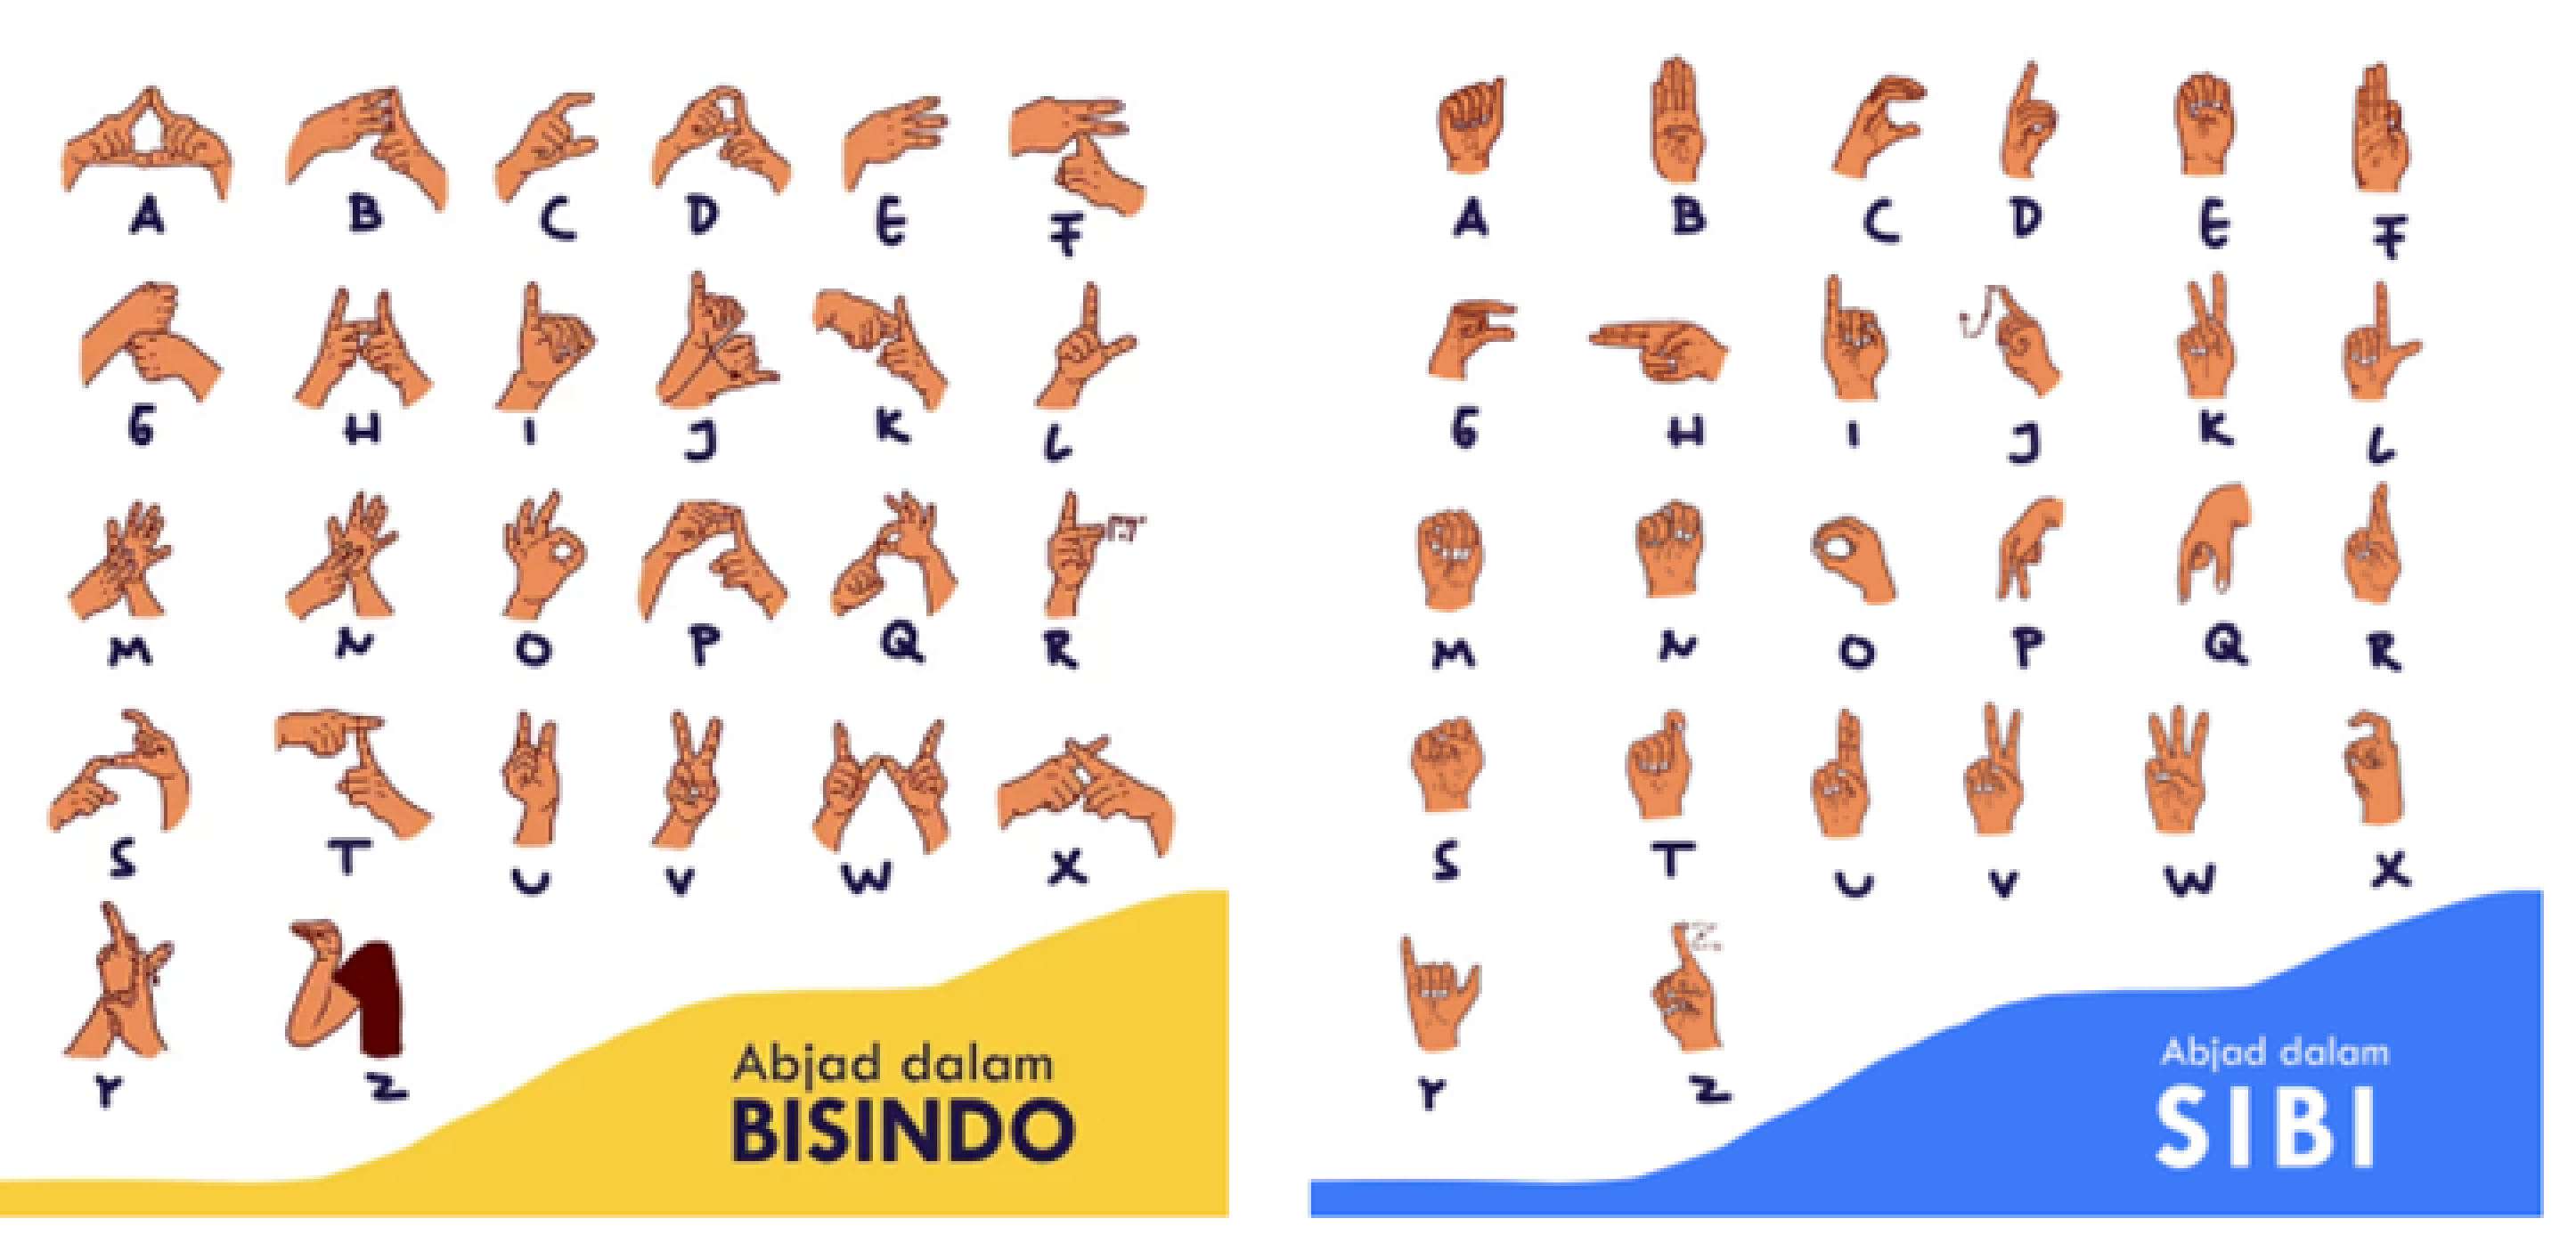
\includegraphics[scale=0.6]{gambar/bab2-isyarat-indonesia.png}
 
%     \caption{Isyarat abjad dalam BISINDO dan SIBI}
%     \label{fig:isyaratindonesia}
% \end{figure}

% Kekurangan pada indra pendengaran yang dialami oleh penyandang tunarungu menyebabkan perkembangan kemampuan berbahasa dan berbicara yang menurun, sehingga banyak dari penyandang tunarungu juga menderita tunawicara. Namun, hal ini bukan menjadi hambatan bagi penderta tunarungu dalam berkomunikasi dengan lingkungan sekitar. Bahasa isyarat adalah bahasa yang dilakukan dengan menggunakan gerakan - gerakan bada yang diiringi dengan ekspresi muka sebagai simbolisasi dari bahasa lisan yang ingin diungkapkan. Tunarungu menggunakan bahasa isyarat sebagai bahasa utama dalam berkomunikasi. Dalam mengungkapkan sesuatu, mereka menggunakan kombinasi antara bentuk tangan, orientasi dan gerak tangan, lengan tubuh, serta ekspresi wajah \parencite{mursita2015}.

% Di Indonesia terdapat 2 bahasa isyarat yang berkembang, yaitu Sistem Bahasa Isyarat Indonesia (SIBI) dan Bahasa Isyarat Indonesia (BISINDO). Berdasarkan gambar \ref{fig:isyaratindonesia}, dapat dilihat bahwa SIBI membentuk isyarat dengan menggunakan 1 tangan saja, sedangkan BISINDO membentuk isyarat menggunakan 2 tangan. BISINDO merupakan isyarat alamiah yang diciptakan dan digunakan sendiri oleh penyandang tunarungu dengan pandangan dan persepsi mereka terhadap segala sesuatu di lingkungan sekitar mereka. Beragam objek atau konsep dapat dinyatakan melalui bahasa isyarat yang mencerminkan bentuk, karakteristik, atau visualnya. Namun, ketika suatu konsep terlalu abstrak untuk direpresentasikan, individu yang tunarungu biasanya akan mengkomunikasikannya dengan memanfaatkan abjad jari \parencite{wedayanti2019}. Tunarungu di Indonesia lebih memilih menggunakan BISINDO sebagai bahasa isyarat yang digunakan dalam kehidupan sehari – hari dibandingkan dengan SIBI karena kemudahan dalam pembentukan isyarat yang tidak terikat pada struktur baku bahasa Indonesia dengan disertai ekspresi wajah dalam pengungkapannya \parencite{handhika2018}. BISINDO sendiri berasal dari bahasa awal atau bahasa ibu tunarungu, dimana penggunaan BISINDO sendiri menyesuaikan dengan pemahaman bahasa tunarungu dari berbagai latar belakang tunarungu dengan tanpa menekankan pada struktur imbuhan bahasa Indonesia \parencite{mursita2015}

% \subsection{MediaPipe}
% MediaPipe merupakan suatu kerangka kerja (\emph{framework}) yang digunakan untuk membantun suatu pipline dalam melakukan inferensi pada data sensorik. MediaPipe memungkinkan untuk membangun suatu pipline yang terdiri dari komponen modular seperti inferensi model, algoritma pemrosesan media, dan transformasi data. Data sensorik seperti audio dan video dapat dimasukkan ke dalam grafik dan menghasilkan \emph{output} berupa deskripsi seperti penentuan objek dan penanda wajah. Kerangka ini mempermudah dalam pembuatan \emph{prototype} cepat dari pipeline persepsi dengan model inferensi dan komponen yang dapat digunakan Kembali. MediaPipe dapat mengabstraksikan dan menghubungkan model – model persepsi individu ke dalam alur yang dapat dipertahankan, dimana hal ini dapat memudahkan dalam penggunaan ulang komponen dalam berbagai aplikasi. Konsep dasar dari MediaPipe terdiri atas tiga bagian utama, yaitu kerangka kerja inferensi data sensorik, seperangkat alat evaluasi kinerja, dan kumpulan komponen inferensi dan pemrosesan yang dapat digunakan kembali. Pipa atau \emph{pipeline} dalam MediaPipe dapat diartikan sebagai grafik komponen yang diarahkan, dimana setiap komponen adalah suatu kalkulator yang spesifik. MediaPipe telah digunakan untuk berbagai aplikasi, termasuk deteksi objek, dan diancang untuk memudahkan dalam pengembangan model machine learning ataupun \emph{ deep learning}, seperti pada deteksi objek dan estimasi pose, terkhususnya pendeteksian gerakan bahasa isyarat \parencite{lugaresi2019:}.

% \subsubsection{Mediapipe Pose}
% Estimasi pose atau pose estimation merupakan suatu aspek yang memiliki peranan penting dalam berbagai teknologi saat ini, seperti mengukur latihan fisik, pengenalan bahasa isyarat, pendeteksian gerakan yoga, menari, dan kebugaran. MediaPipe pose terinspirasi oleh model BlazeFace yang digunakan dalam deteksi wajah Mediapipe, sebagai proksi untuk mendeteksi orang. Model ini dapat dikatakan terinspirasi oleh Virtuvian Leonardo, untuk memperkirakan titik Tengah pinggul seseorang, jari – jari lingkaran yang mengelilingin seluruh orang, dan sudut kemiringan garis yang menghubungkan titik tengah bahu dan pinggul. Model \emph{landmark} dari Mediapipe pose ini memprediksi total 33 lokasi \emph{landmark}, dengan diawali dari bagian hidung hingga diakhiri pada kaki bagian kanan \parencite{googleMediapipe}. 

% \begin{figure}[H]
%     \centering

%     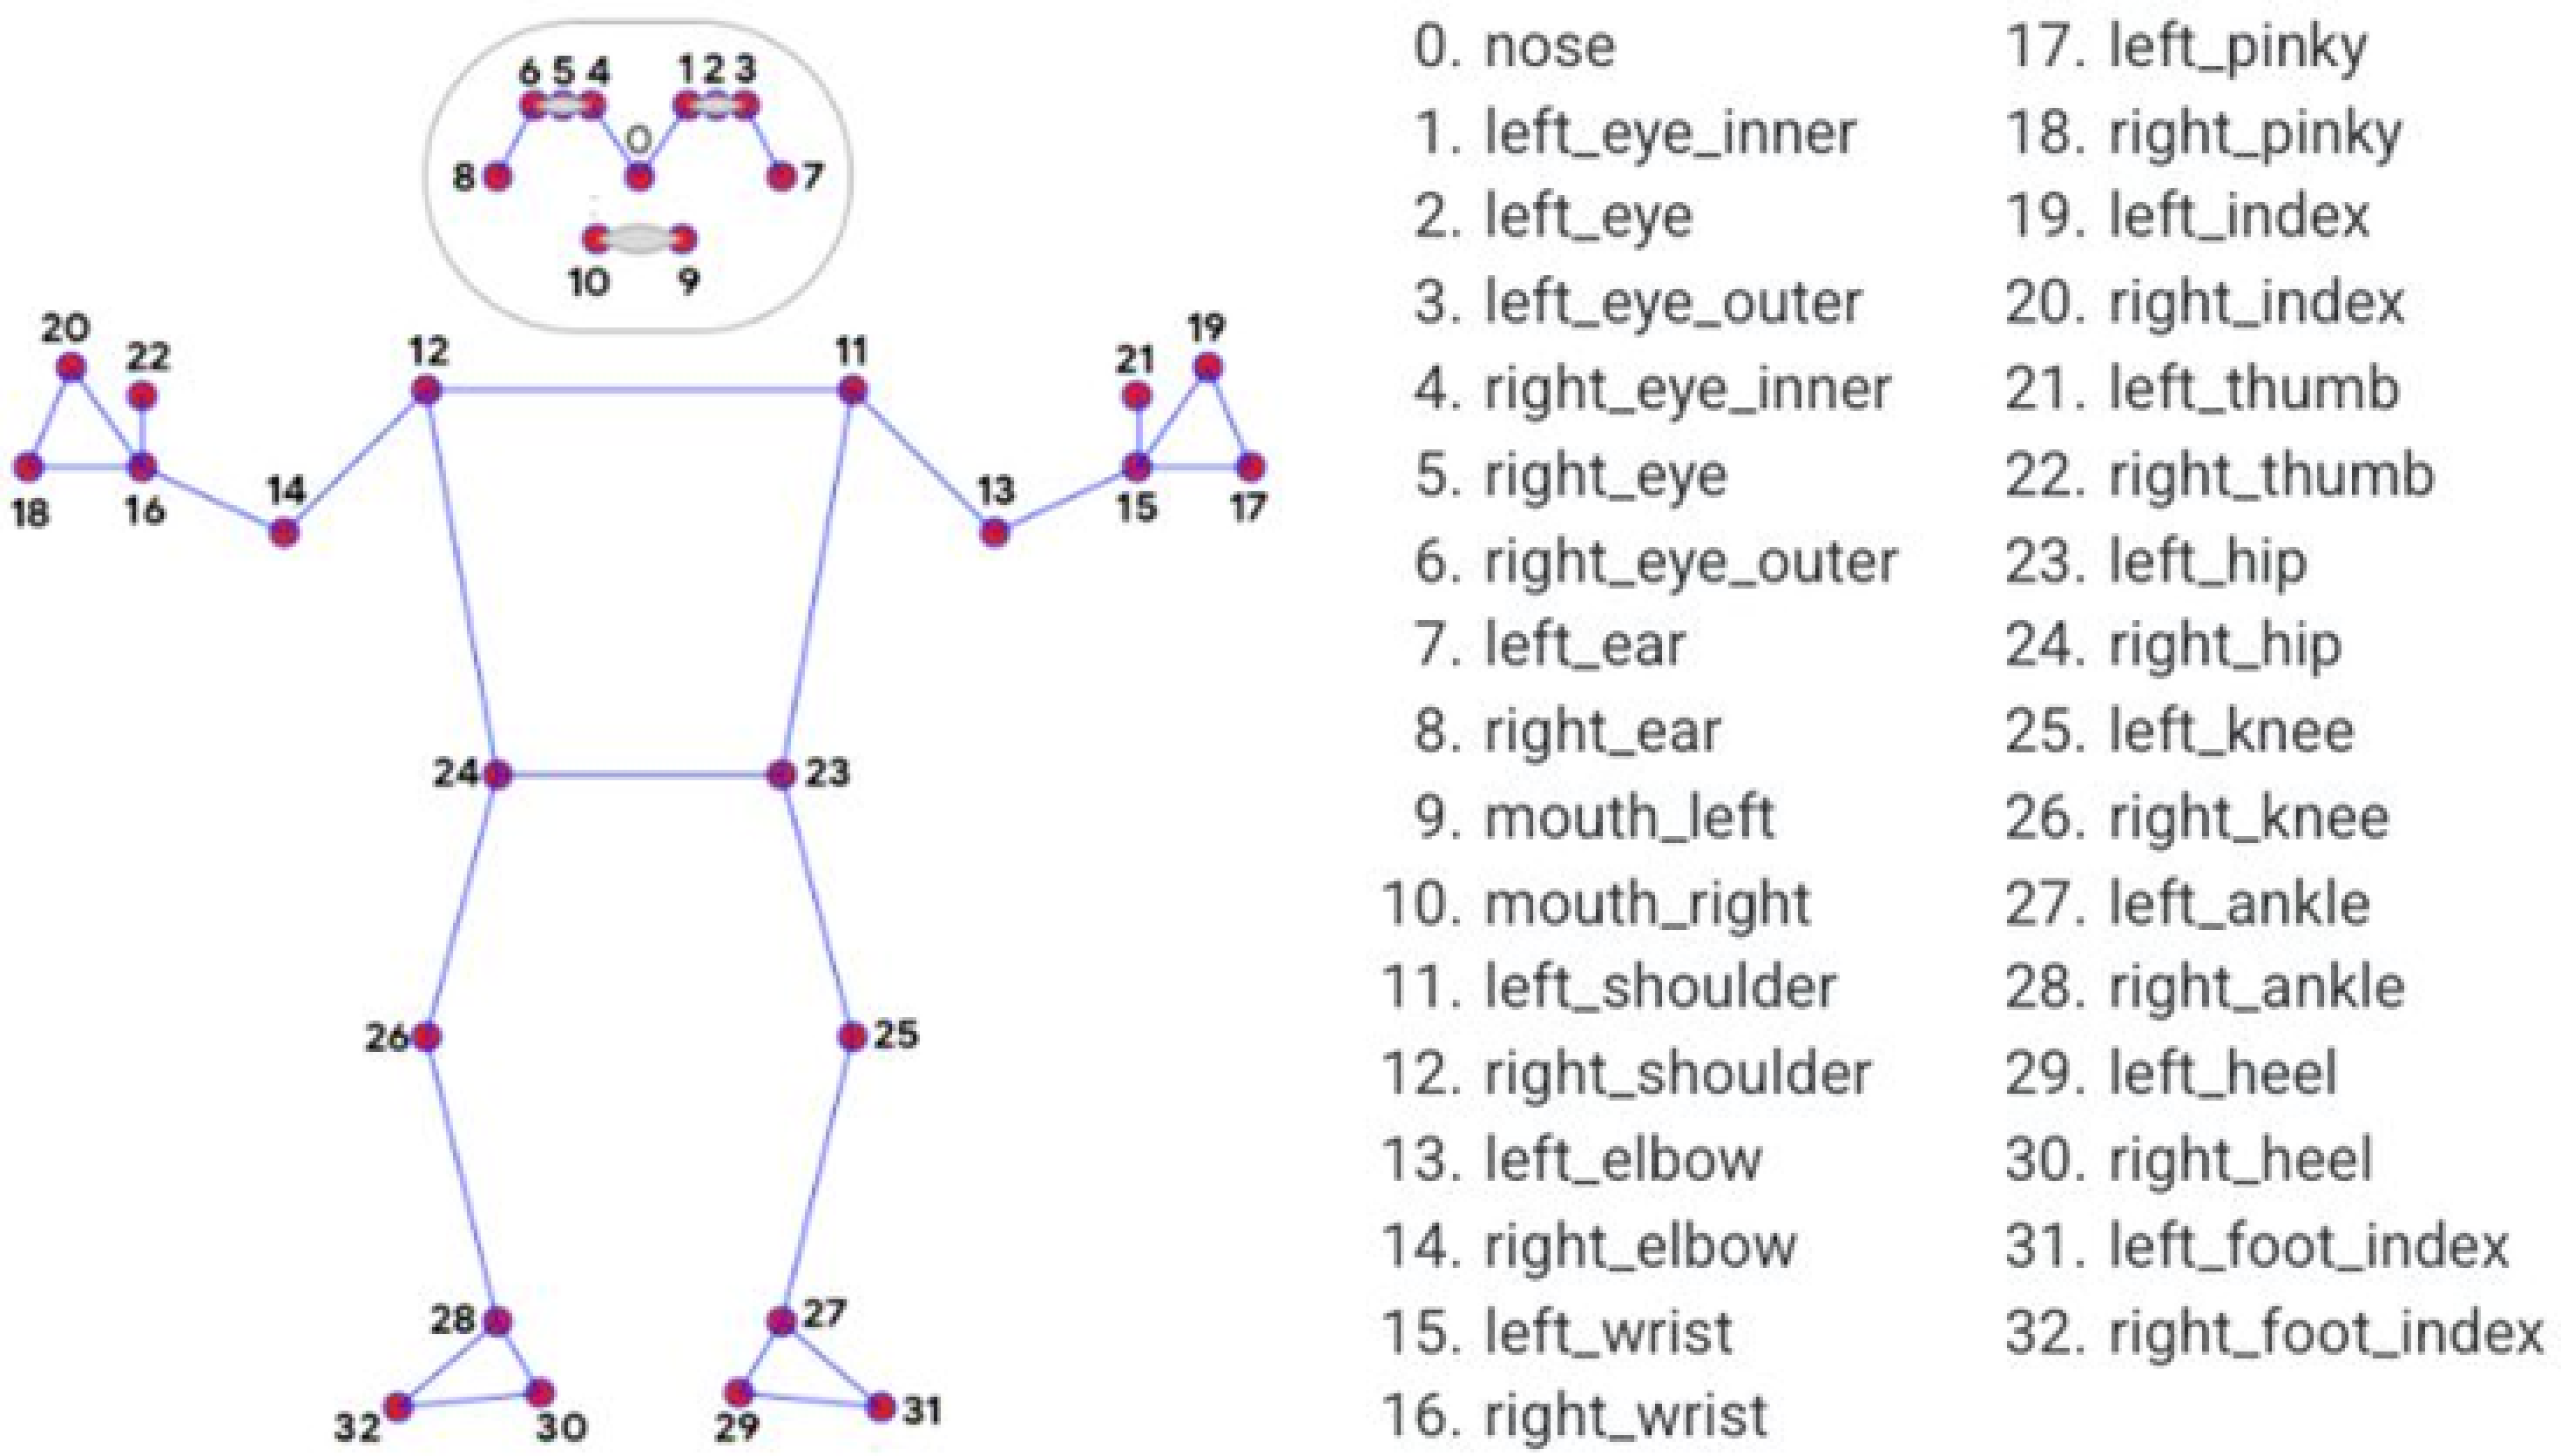
\includegraphics[scale=0.5]{gambar/bab2-mp-pose.png}
 
%     \caption{\textit{Keypoints} \emph{landmark}s pada MediaPipe pose}
%     \label{fig:mediapipepose}
% \end{figure}

% \subsubsection{Mediapipe Hand}
% Kemampuan untuk merasakan bentuk dan gerakan tangan dapat menjadi komponen penting dalam meningkatkan pengalaman pengguna di berbagai platform teknologi, seperti pendeteksian gerakan tangan pada pembentukan bahasa isyarat yang memiliki artinya masing – masing. MediaPipe hand adalah solusi pelacakan tangan dan jari dengan ketelitian tinggi dengan menggunakan \textit{machine learning} untuk menyimpulkan 21 \emph{landmark} 3D tangan dari satu bingkai. Pada setiap ruas jari memiliki \emph{landmark}-nya tersendiri sehingga total \emph{landmark} dari 4 \emph{landmark} dan untuk pangkal telapak tangan terdapat 1 buah \emph{landmark} \parencite{googleMediapipe}.

% \begin{figure}[H]
%     \centering

%     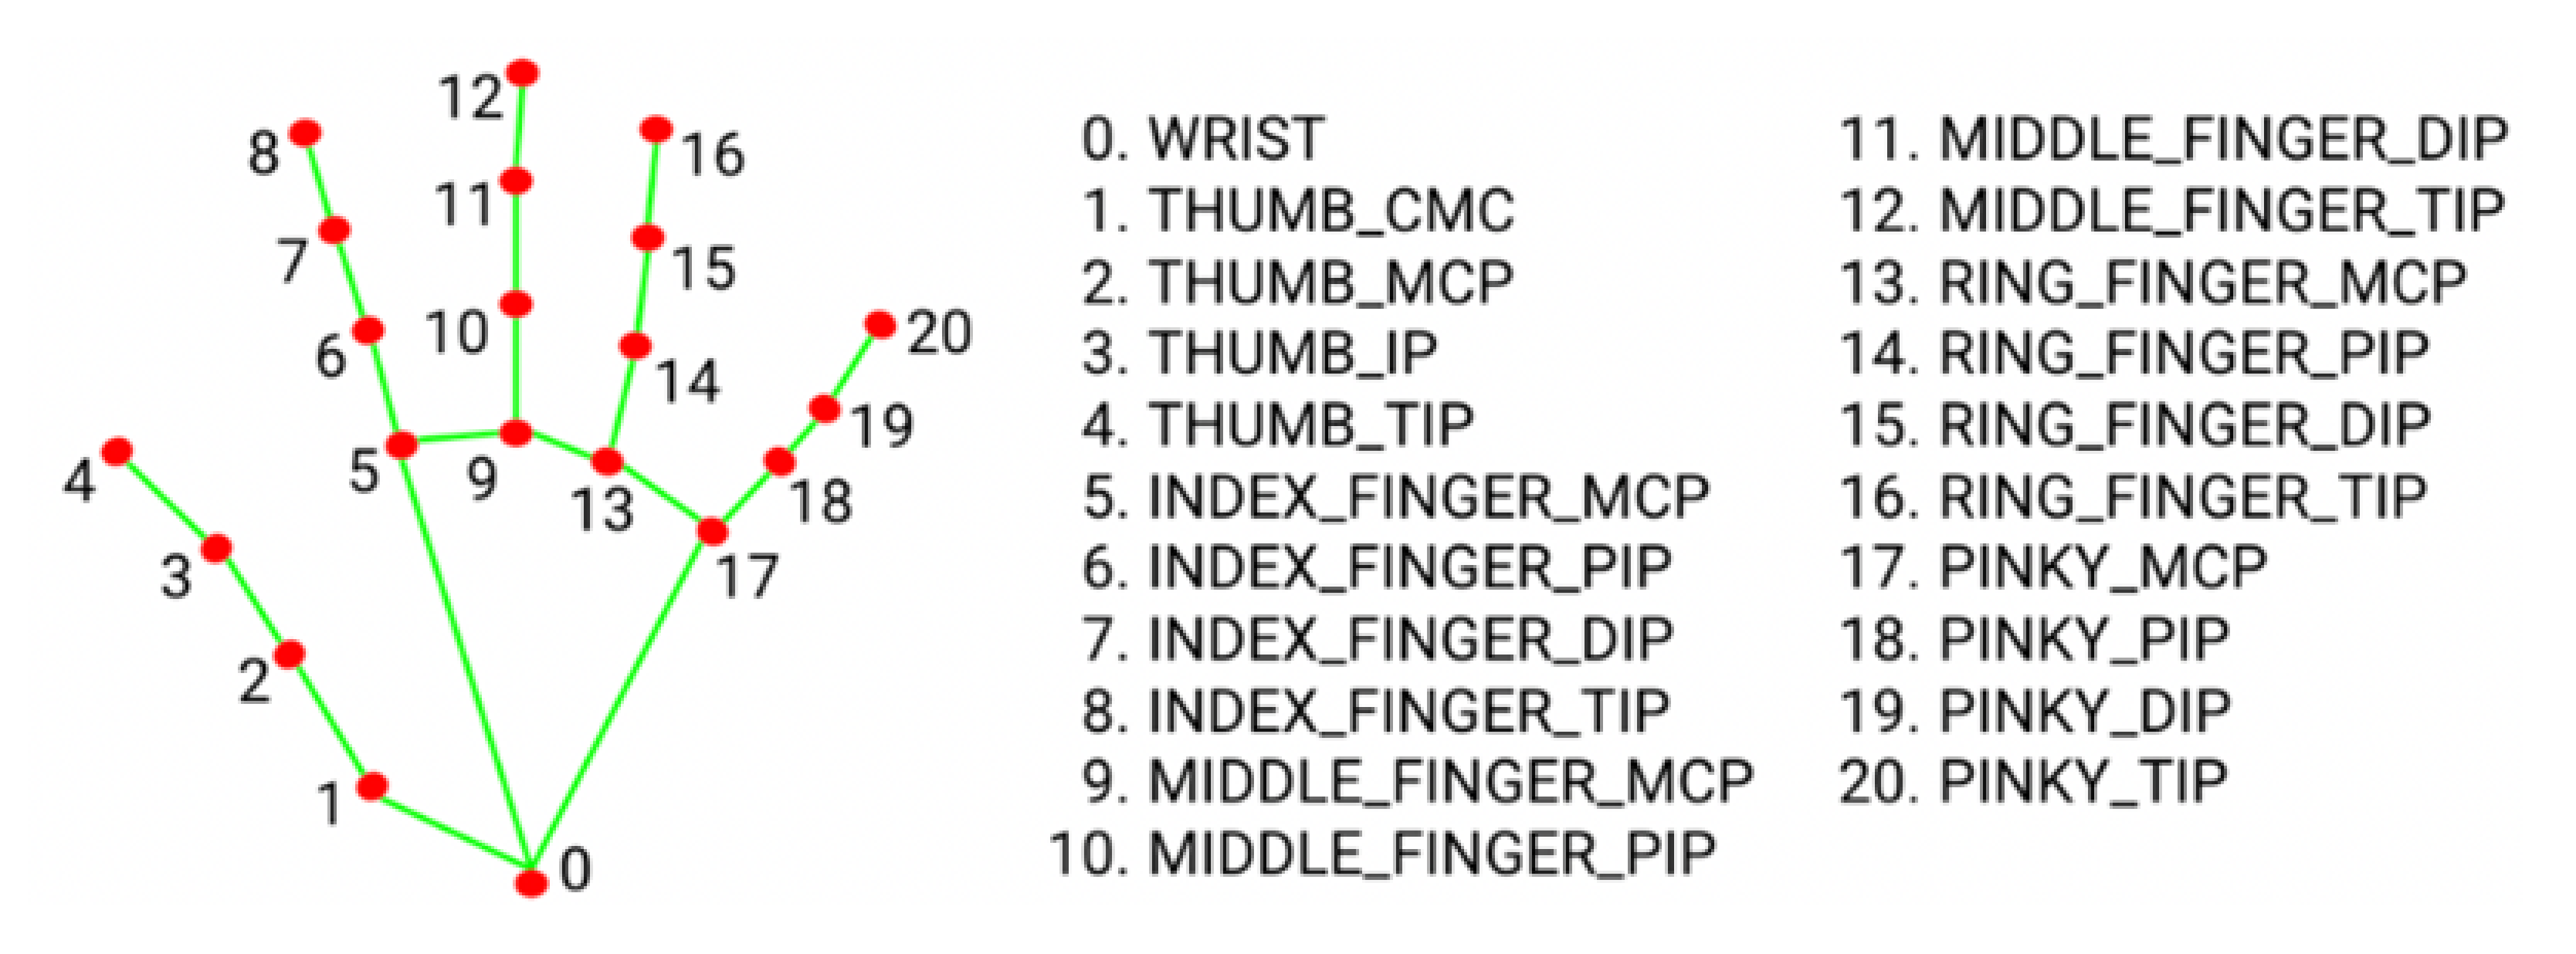
\includegraphics[scale=0.5]{gambar/bab2-mp-hand.png}
 
%     \caption{\textit{Keypoints} \emph{landmark}s pada MediaPipe Hand}
%     \label{fig:mediapipehand}
% \end{figure}

% \subsection{\textit{Long Short-Term Memory} (LSTM)}

% \begin{figure}[H]
%     \centering

%     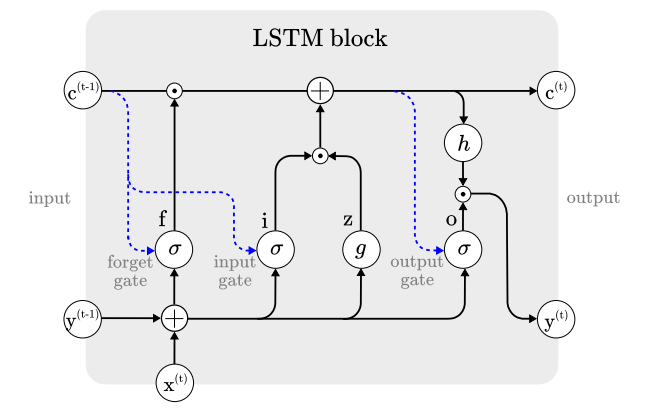
\includegraphics[scale=1.2]{gambar/bab2-lstm-model.png}
 
%     \caption{Cara kerja arsitektur LSTM}
%     \label{fig:longshortterm}
% \end{figure}

% \textit{Long Short-Term Memory} (LSTM) merupakan bentuk khusus dari neural network RNN atau \textit{Recurrent Neural Network} yang memiliki kemampuan \textit{feedback connection}. Kemampuan ini memungkinkan LSTM untuk dapat mengingat informasi untuk waktu yang lama sehingga dapat digunakan untuk menyelesaikan permasalahan yang memiliki sifat sekuensial atau berurutan. Keunggulan LSTM jika dibandingkan dengan RNN adalah LSTM memiliki kemampuan untuk mengingat informasi yang lebih baik dan efektif sehingga meminimalisir terjadinya kehilangan informasi yang umum terjadi pada pemrosesan informasi lama yang panjang pada penggunaan RNN \parencite{xia2020}. Oleh karena itu, LSTM cocok untuk dimanfaatkan dalam pengembangan suatu sistem penerjemah isyarat yang mana membutuhkan kemampuan dalam mengingat gerakan bahasa isyarat yang bersifat sekuensial untuk kemudian disimpan dan diterjemahkan ketika terdapat gerakan yang sesuai.

% Pada gambar \ref{fig:modelLSTM}, \textit{Long Short-Term Memory} tersusun atas beberapa layer yang meliputi \textit{block input}, \textit{input gate}, \textit{forget gate}, \textit{cell}, \textit{output gate}, dan \textit{block output}. \textit{Block input} bertindak untuk melakukan pembaharuan terhadap $x^{(t)}$ dengan \textit{Block input} LSTM unit $y^{(t-1)}$ pada iterasi terakhir. Hal ini dapat dirumuskan sebagai berikut:

% \begin{equation}
%   \label{eq:blockinputLSTM}
%   x^{(t)} = g(W_z x^{(t)} + R_z y^{(t-1)} + b_z)
% \end{equation}

% Pada rumus \ref{eq:blockinputLSTM}, $W_z$ dan $R_z$ merupakan \textit{weight} yang diasosiasikan dengan $x^{(t-1)}$ dan $y^{(t-1)}$ secara berurutan. Sedangkan $b_z$ diartikan sebagai \textit{weight bias vector}. Paada \textit{layer} ini, LSTM   Pada input gate, akan dilakukan pembaharuan terhadap \textit{input} saat ini, ($x^{(t)}$), \textit{output} dari unit LSTM ($y^{(t-1)}$), dan nilai dari \textit{cell} ($c^{(t-1)}$) pada iterasi terakhir. Hal ini  dapat dirumuskan sebagai:

% \begin{equation}
%     \label{eq:inputgateLSTM}
%     i^{(t)} = \sigma(W_i x^{(t)} + R_i y^{(t-1)}+ p_i \odot c^{(t-1)} + b_i)
% \end{equation}

% Pada rumus \ref{eq:inputgateLSTM}, $\odot$ melambangkan perkalian titik antara 2 buah vector. $W_i$, $WR_i$, dan $p_i$ adalah weight yang dimiliki oleh $x^{(t)}$, $y^{(t-1)}$, dan $c^{(t-1)}$. Sementara $b_i$ merepresentasikan bias vector yang diasosasikan oleh unit ini. Forget gate bertindak untuk menentukan informasi yang harus dihapus dari \textit{cell state} ($c^{(t-1)}$) sebelumnya. Oleh karena itu, nilai fungsi aktivasi dari \textit{forget gates} pada \textit{time step} t dihitung berdasarkan input saat ini ($x^{(t)}$), \textit{ouput} ($y^{(t - 1)}$), \textit{state memory cell} ($y^{(t - 1)}$) pada \textit{time step} sebelumnya ($t - 1$), koneksi \textit{peephole}, dan \textit{bias} dari \textit{forget gate} itu sendiri (${b_f}$). \textit{Forget gate} dapat dirumuskan sebagai:

% \begin{equation}
%     \label{eq:forgetgateLSTM}
%     f^{(t)} = \sigma(W_f x^{(t)} + R_f y^{(t-1)}+ p_f \odot c^{(t-1)} + b_f)
% \end{equation}

% Pada rumus \ref{eq:forgetgateLSTM}, $W_f$, $R_f$, dan $p_f$ adalah \textit{weight} yang diasosiasikan dengan $x^{(t)}$, $y^{(t-1)}$, dan $c^{(t-1)}$. Sementara $b_i$ merepresentasikan bias vector yang diasosasikan oleh unit ini. \textit{Cell} merupakan bagian yang melakukan komputasi untuk nilai dari \textit{cell} itu sendiri yang merupakan gabungan dari nilai - nilai pada input $z^{(t)}$, input gate $i^{(t)}$, dan \textit{forget gate} $f^{(t)}$ dengan nilai pada \textit{cell} sebelumnya. Hal ini dapat dirumuskan sebagai:

% \begin{equation}
%     \label{eq:cellLSTM}
%     c^{(t)} =  z^{(t)} \odot  i^{(t)} + z^{(t-1)} \odot  f^{(t)}
% \end{equation}

% Pada \textit{output gate}, akan dilakukan perhitungan untuk \textit{input} saat ini $x^{(t)}$, \textit{output} dari LSTM unit $y^{(t-1)}$, dan nilai cell $c^{(t-1)}$ pada iterasi terakhir. Hal ini dapat dirumuskan sebagai:

% \begin{equation}
%     \label{eq:outputgateLSTM}
%     o^{(t)} = \sigma(W_o x^{(t)} + R_o y^{(t-1)}+ p_o \odot c^{(t)} + b_o)
% \end{equation}

% Pada rumus \ref{eq:outputgateLSTM}, $W_f$, $R_f$, dan $p_f$ adalah\textit{weight} yang diasosiasikan dengan $x^{(t)}$, $y^{(t-1)}$, dan $c^{(t-1)}$. Sementara $b_i$ merepresentasikan \textit{bias vector} yang diasosasikan oleh unit ini. Pada \textit{block otuput}, akan dihitung nilai \textit{cell} saat ini $(c^{(t)})$ dengan nilai output gate saat ini. Hal ini dapat dirumuskan sebagai berikut:

% \begin{equation}
%     \label{eq:blockoutputLSTM}
%     c^{(t)} =  g(c^{(t)}) \odot o^{(t)}
% \end{equation}

% Pada persamaan - persamaan diatas, $\sigma$, $g$, $h$ melambangkan fungsi aktivasi non-linear antar titik. Fungsi logistik \textit{sigmoid} $(\sigma(x) = \frac{1}{1 + e^{-x}})$ digunakan sebagai fungsi aktivasi pada \textit{gate}. Sedangkan fungsi aktivasi \textit{hyperbolic} tangent $g(x) = h(x) = tanh(x)$ digunakan seabagai aktivasi fungsi pada \textit{block input} dan \textit{output} \parencite{van2020}.

% \subsection{Intel \emph{Next Unit Computing} (NUC)}

% \begin{figure}[H]
%     \centering

%     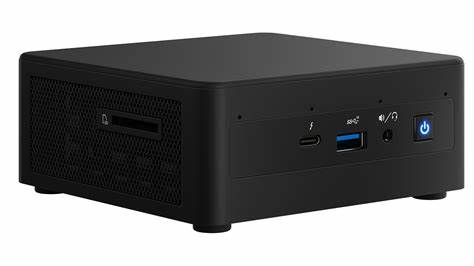
\includegraphics[scale=0.6]{gambar/bab2-nuc_11_performace_kit.jpeg}
 
%     \caption{Intel NUC 11 \emph{Performance Kit}}
%     \label{fig:jetsonnano}
% \end{figure}

% Intel \emph{Next Unit Computing} (NUC) merupakan komputer \emph{barebone} dengan ukuran kecil yang dirancang oleh Intel. Intel NUC merupakan perangkat yang berfokus dalam menyediakan komputasi kuat dalam ukuran yang praktis dan dapat melayani berbagai kebutuhan pengguna, mulai dari bermain \emph{game}, bisnis, hingga menjalankan aplikasi kompleks. Intel NUC secara resmi memperkenalkan perangkat ini pada tahun 2012 dan dipasarkan secara umum pada awal tahun 2013 \parencite{IntelNUC2020}. Adapun seri pertama dari Intel NUC memiliki CPU Sandy Bridger berbasis Celeron. Intel NUC telah berkembang hingga generasi ke-12 bernama Dragon Canyon yang dilengkapi dengan CPU Intel generasi ke-12 dan PCI Express Gen 5 \parencite{Halfacree2013}.

% Intel NUC 11 merupakan perangkat Intel yang dirilis pada 13 Januari 2021 dengan kode nama Phantom Canyon. Salah satu model yang cukup banyak digunakan adalah Intel NUC 11 Performance Kit model NUC11PAHi7. Inti dari perangkat ini dilengkapi dengan prossesor Intel Core i7-1165G7. Prossesor ini memiliki quad-core yang memiliki kecepatan dasar 2.8 GHz dan dapat meningkat hingga 4.7 GHz.  Prossesor ini didukung oleh kartu grafis Iris XE yang menawarkan peningkatan kinerja grafis yang substansial dibandingkan dengan generasi sebelumnya. Hal ini memudahkan perangkat dalam menjalankan tugas mulai dari pengeditan video hingga bermain \emph{game}. Dari segi memori, Intel NUC 11 Performance Kit model NUC11PAHi7 mendukung hingga 64GB DDR4-3200 SODIMM dual-channel, menyediakan ruang yang luas untuk multitasking intensif. Untuk penyimpanan, perangkat ini menawarkan slot M.2 yang fleksibel yang mendukung SSD NVMe terbaru dengan memastikan kecepatan akses dan penyimpanan data yang cepat. Hal ini kritikal untuk aplikasi yang melibatkan set data besar atau pemrosesan \emph{realtime}. Konektivitas adalah salah satu kekuatan utama model ini, menampilkan berbagai pilihan termasuk Thunderbolt 4, HDMI 2.0b, dan beberapa port USB 3.1. Ini memungkinkan koneksi banyak periferal dan tampilan secara bersamaan, meningkatkan produktivitas dan fleksibilitas dalam skenario penggunaan. Selain itu, dengan Intel Wi-Fi 6 dan Bluetooth 5.1, Intel NUC 11 pada model ini menawarkan konektivitas nirkabel terdepan untuk integrasi yang mulus ke dalam lingkungan jaringan apa pun. Dimensi yang ringkas untuk model ini NUC11PAHi70Z, yang hanya berukuran 117 x 112 x 51 mm dapat menjadikannya pilihan ideal untuk lingkungan di mana ruang terbatas \parencite{ASUS2024}. Kombinasi komputasi berkinerja tinggi, kemampuan grafis yang kuat, dan opsi konektivitas yang luas, semua dalam bentuk yang kecil, menonjolkan NUC11PAHi70Z sebagai pilihan teratas bagi pengguna yang membutuhkan solusi komputasi yang kuat, serbaguna, dan efisien ruang.

% % \subsection{Jetson Nano}
% % \begin{figure}[H]
% %     \centering

% %     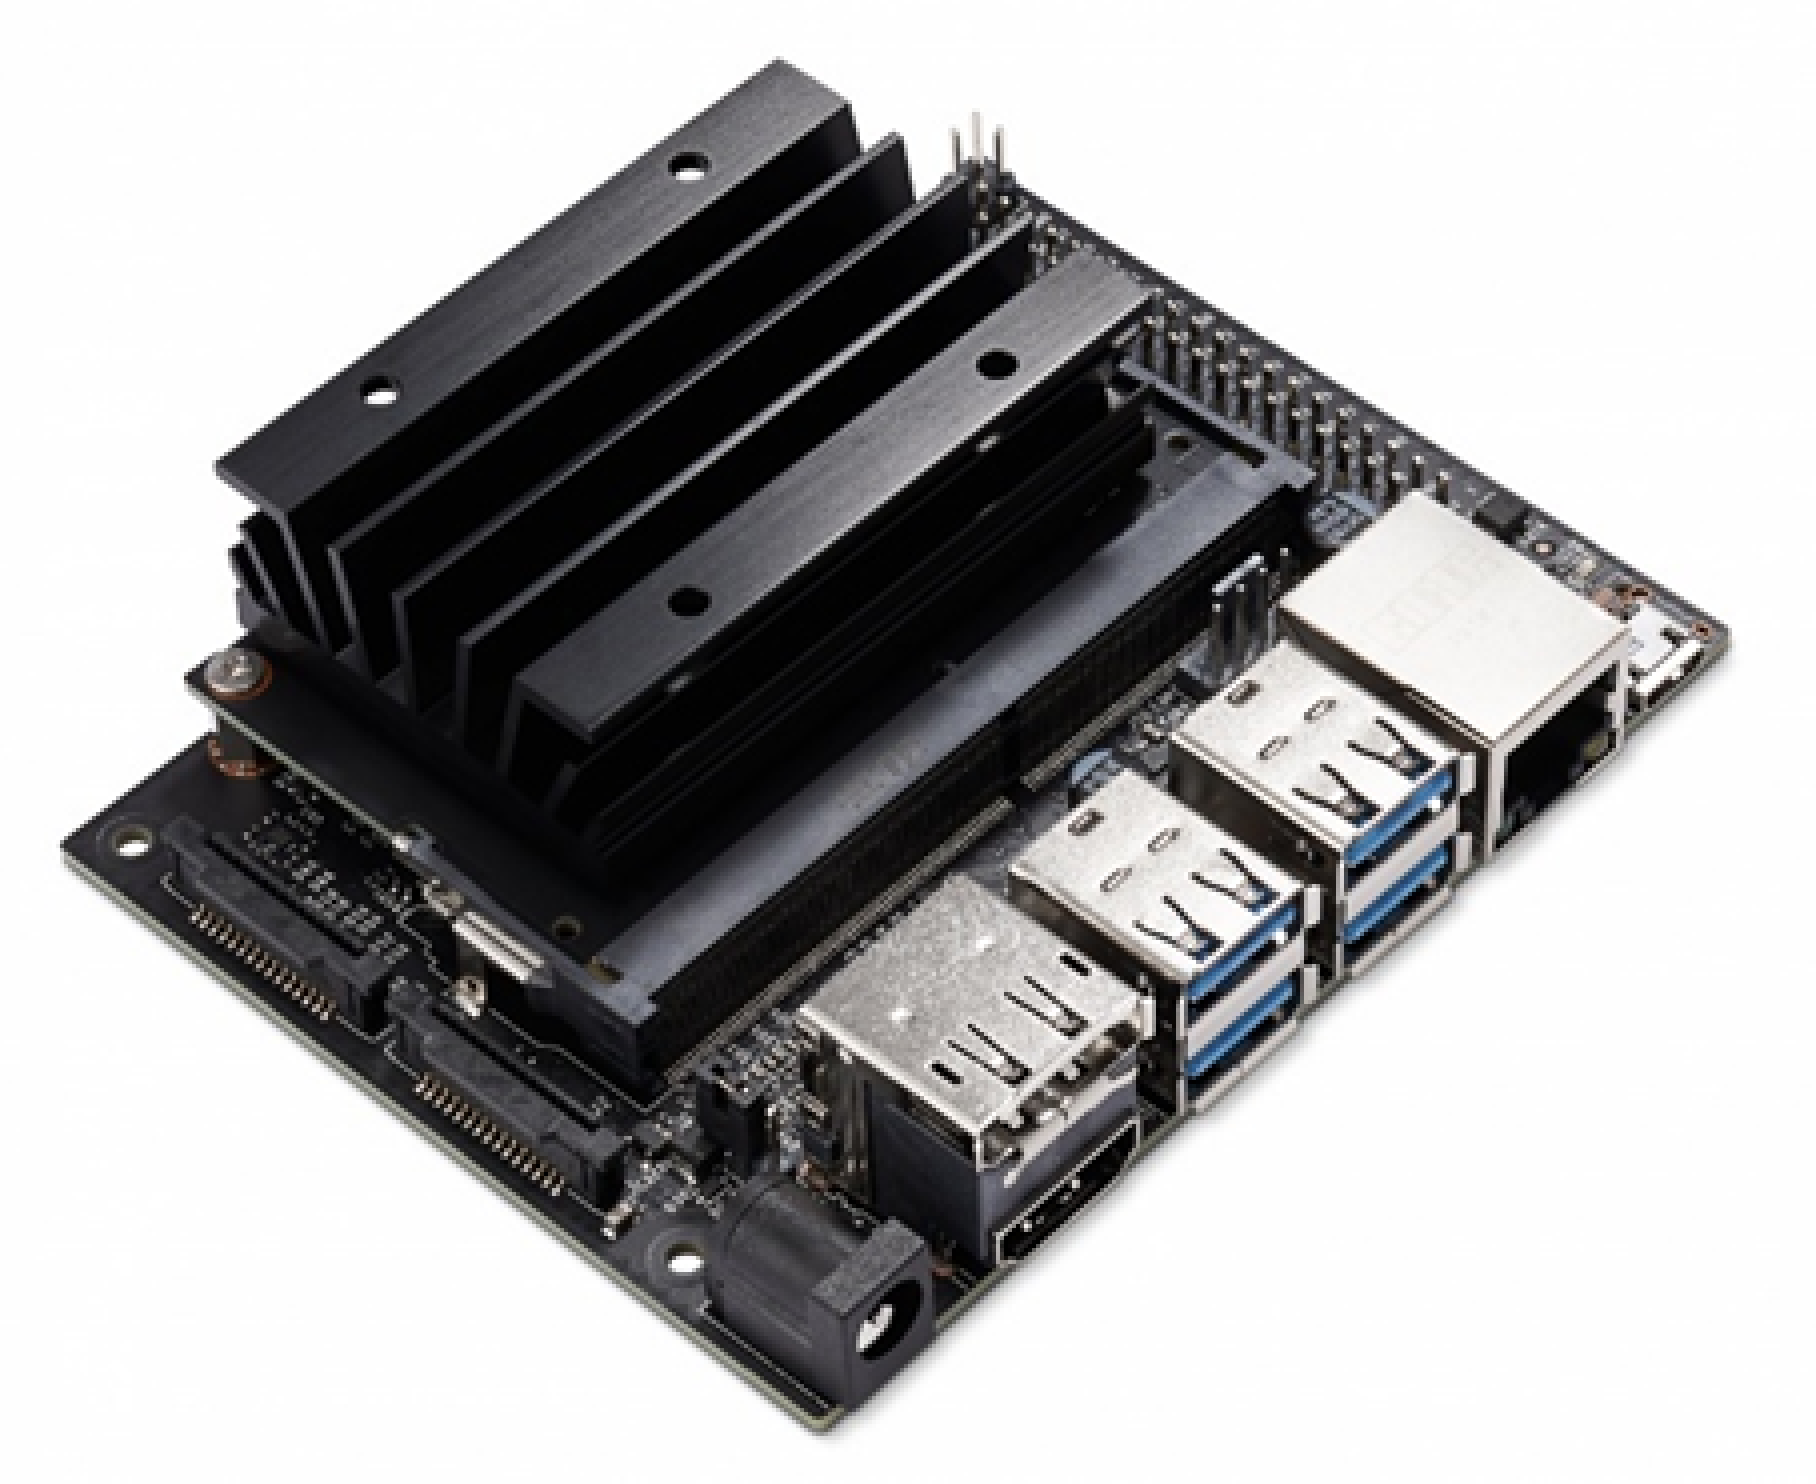
\includegraphics[scale=0.6]{gambar/bab2-jetson-nano.png}
 
% %     \caption{Jetson Nano Developer Kit}
% %     \label{fig:jetsonnano}
% % \end{figure}

% % Jetson Nano adalah perangkat komputasi keluaran NVIDIA yang didedikasikan dalam pengembangan \textit{machine lerarning} dan komputasi edge. Jetson Nano memiliki kemampuan untuk dapat menjalankan beberapa neural networks secara paralel. Kemampuan ini memungkinkan Jetson Nano untuk digunakan dalam \textit{image clasiification}, \textit{object detection}, \textit{segmentation}, dan \textit{speech processing} \parencite{nvidiaJetsonNano}. Perangkat ini dapat menjadi solusi dalam menjalankan model \textit{machine learning} atau \textit{deep learning} pada perangkat portable dan hemat energi. 

% % Perangkat ini dilengkapi dengan 128 NVIDIA CUDA cores. Ditenagai oleh prosesor Quad-core ARM Cortex-A57 MPCore, platform ini menyediakan fungsionalitas komputasi yang solid dengan memori 4 GB 64-bit LPDDR4 yang beroperasi pada 1600MHz, memberikan bandwidth 25.6 GB/s. Untuk penyimpanan, Jetson Nano dilengkapi dengan 16 GB eMMC 5.1, yang memberikan ruang yang cukup untuk aplikasi dan data pengguna. Dalam konteks pengkodean video, perangkat ini dapat mengkodekan video dengan kecepatan 250MP/sec, mendukung format seperti 1x 4K pada 30fps (HEVC), 2x 1080p pada 60fps (HEVC), dan sebagainya. Sementara itu, untuk decode video, perangkat ini menawarkan kemampuan hingga 500MP/sec, dengan dukungan untuk format seperti 1x 4K pada 60fps (HEVC) dan 2x 4K pada 30fps (HEVC). Jetson Nano juga dilengkapi dengan 12 jalur kamera (3x4 atau 4x2) MIPI CSI-2 D-PHY 1.1, yang mendukung kecepatan hingga 1.5 Gb/s per pasangan, memberikan fleksibilitas dalam pengembangan aplikasi berbasis kamera. Dalam hal konektivitas, perangkat ini menawarkan Gigabit Ethernet dan M.2 Key E, serta kemampuan tampilan melalui HDMI 2.0 dan eDP 1.4. Jetson Nano juga dilengkapi dengan 4x USB 3.0 dan USB 2.0 Micro-B, serta berbagai opsi konektivitas lainnya seperti GPIO, I2C, I2S, SPI, dan UART, semuanya dalam form factor mekanis 69.6 mm x 45 mm dengan konektor tepi 260-pin \parencite{nvidiaJetsonNano}.

% \subsection{Performa Klasifikasi}

% \begin{figure}[H]
%     \centering

%     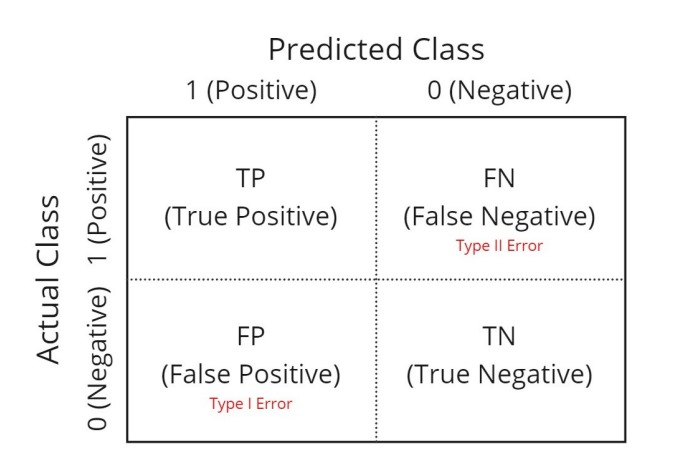
\includegraphics[scale=0.8]{gambar/bab2-confusion-matrix.png}
 
%     \caption{\textit{Confusion matrix}}
%     \label{fig:confusionMatrix}
% \end{figure}

% Dalam melakukan klasifikasi dengan model, diperlukan adanya suatu tolak ukur berdasarkan serangkaian dataset pengujian yang diberikan. Salah satu metode yang dapat digunakan adalah dengan menggunakan \textit{confusion matrix}. \textit{Confusion matrix} merupakan sebuah konsep yang umum digunakan dalam menentukan performa klasifikasi model dengan memberikan informasi mengenai data aktual dan data prediksi model klasifikasi. Berdasarkan \ref{fig:confusionMatrix} \textit{confusion matrix} memiliki bentuk matrix 2 dimensi, dimana satu dimensi memiliki index yang berisikan data aktual dari \textit{class} obyek klasifikasi dan satu dimensi lainnya memiliki index yang berisikan data klasifikasi yang dihasilkan oleh model \parencite{deng2016}. 

% Pada \textit{confusion matrix}, terdapat empat aspek yang digunakan untuk merepresentasikan perbandingan dari kelas aktual dan kelas prediksi. Keempat aspek tersebut meliputi \textit{true positive}, \textit{true negative}, \textit{false positive}, \textit{true negative}. \textit{True positive} (TP) merupakan kondisi dimana data aktual bernilai 1 (positif) diprediksi sebagai data yang bernilai 1 (positif). Sedangkan \textit{true negative} (TN) merupakan kondisi dimana data aktual bernilai 0 (negatif) diprediksi sebagai data yang bernilai 0 (negatif). \textit{False positive} (FP) merupakan kondisi dimana data aktual bernilai 0 (negatif) diprediksi sebagai data yang bernilai 1 (positif). Sedangkan \textit{false negative} (TN) merupakan kondisi dimana data aktual bernilai 1 (positif) diprediksi sebagai data yang bernilai 0 (negatif) \parencite{shajihan2020}. Keempat aspek ini kemudian dapat dihitung nilai \textit{accuracy}, \textit{precision}, \textit{recall}, \textit{F-score} yang dapat membantu dalam memahami performa klasifikasi model dengan lebih detail lagi.

% \subsubsection{\textit{Accuracy}}
% \textit{Accuracy} merupakan metode untuk mengevaluasi kinerja yang menunjukkan tingkat ketep\\atan sebuah model dalam mengklasifikasikan data pengujian yang diberikan secara akurat. \textit{Accuracy} dapat diartikan sebagai perbandingan antara prediksi benar (TP dan TN) terhadap keseluruhan data yang ada. Secara sederhana, \textit{accuracy} menggambarkan seberapa dekat nilai prediksi berada dengan nilai sebenarnya. \textit{Accuracy} dapat dirumuskan dirumuskan pada persamaan \ref{eq:perofrmaAccuracy} \parencite{OvalleMagallanes2020}
   
% \begin{equation}
%     \label{eq:perofrmaAccuracy}
%     Accuracy = \frac{TP + TN}{TP + TN + FP + FN}
% \end{equation}

% \subsubsection{\textit{Precision}}
% \textit{Precision} merupakan metode untuk mengevaluasi kinerja yang mengukur seberapa akurat data yang diminta cocok dengan hasil prediksi yang diberikan oleh model. \textit{Precision} dapat diartikan sebagai perbandingan antara prediksi benar positif (TP) terhadap total hasil yang diprediksi positif (jumlah TP dan FP). \textit{Precision} dapat irumuskan pada persamaan \ref{eq:perofrmaPrecision} \parencite{OvalleMagallanes2020}

% \begin{equation}
%     \label{eq:perofrmaPrecision}
%     Precision = \frac{TP}{TP + FP}
% \end{equation}

% \subsubsection{\textit{Recall}}
% \textit{Recall} merupakan metode untuk menunjukkan kemampuan sebuah model untuk secara akurat mengidentifikasi informasi yang relevan. Recall dapat diartikan sebagai perbandingan antara umlah prediksi benar positif (TP) dengan total jumlah data aktual positif (jumlah TP dan FN). \textit{Recall} dapat dirumuskan pada persamaan \ref{eq:perofrmaRecall} \parencite{OvalleMagallanes2020}

% \begin{equation}
%     \label{eq:perofrmaRecall}
%     Recall = \frac{TP}{TP + FN}
% \end{equation}

% \subsubsection{\textit{F-Score}}

% \textit{F-Score} adalah nilai yang berkisar antara nol hingga satu yang diperoleh dari rata - rata tertimbang (\textit{harmonic mean}) antara nilai precision dan recall. \textit{F-Score} dapat dirumuskan pada persamaan \parencite{Deng2016}

% \begin{equation}
%     \label{eq:perofrmaFScore}
%     F{-}Score = \frac{2 \times {Precision} \times {Recall}}{{Precision} + {Recall}}
% \end{equation}

% \label{subsec:hukumnewton}

% Newton \parencite{newton1687} pernah merumuskan bahwa \lipsum[1]
% Kemudian menjadi persamaan seperti pada persamaan \ref{eq:hukumpertamanewton}.

% Contoh pembuatan persamaan
% \begin{equation}
%   \label{eq:hukumpertamanewton}
%   \sum \mathbf{F} = 0\; \Leftrightarrow\; \frac{\mathrm{d} \mathbf{v} }{\mathrm{d}t} = 0.
% \end{equation}

% \subsection{Anti Gravitasi}
% \label{subsec:antigravitasi}

% Anti gravitasi merupakan \lipsum[1]


% % Contoh input gambar
% \begin{figure}[H]
%   \centering

%   % Ubah dengan nama file gambar dan ukuran yang akan digunakan
%   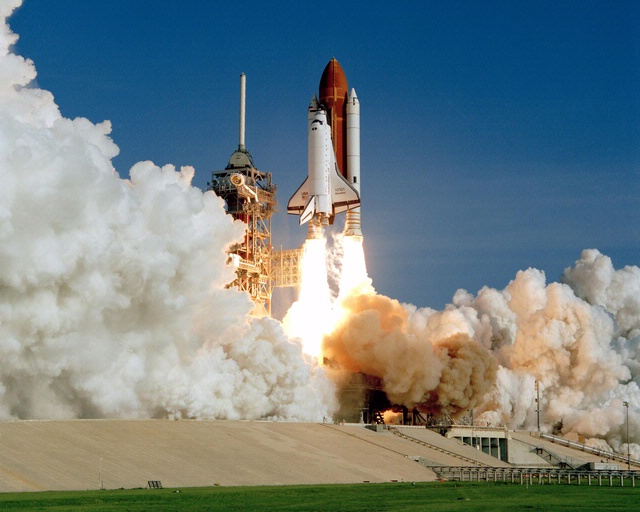
\includegraphics[scale=0.35]{gambar/roketluarangkasa.jpg}

%   % Ubah dengan keterangan gambar yang diinginkan
%   \caption{Peluncuran roket luar angkasa \emph{Discovery} \parencite{roketluarangkasa}.}
%   \label{fig:roketluarangkasa}
% \end{figure}

% Roket luar angkasa merupakan \lipsum[1]

% \emph{Discovery}, Gambar \ref{fig:roketluarangkasa}, merupakan \lipsum[2]